In the PyMarl framework, we must define an agent network (which is a neural network architecture that each agent uses to determine $Q$-values) and a mixing network, which takes each agent's $Q$-value to produce a total $Q$-value, $Q_total$. Note the difference between an agent and an agent network: an agent is one of many actors within the multi-agent system, whereas the agent network is the neural network architecture that makes up the $Q$-value function of each agent. Furthermore, in this project, every agent uses the same neural network. We will fix the mixing network to either VDN or QMIX, as these have been shown to have good performance in previous tests. 


Each agent network takes the form of a neural network to approximate the state-value function, which takes an input (a tensor) consisting of an observation (and possibly a particular action). To avoid unnecessary overheads, we pass the input for every agent and batch element as one large tensor (note that every agent's observation is passed through the same neural network), so that PyTorch can perform the feedforward just once, and gets an appropriate tensor of $Q$ values as output. Concretely, if there are $n$ agents, we have a batch size of $b$, and each observation has size $o$, then the input tensor has shape $(n\times b, o)$, while the output tensor of $Q$ values has size $(n \times b, a, 1)$, where $a$ is the number of actions. Conversely, if the agent network takes actions as input also (and gives a single $Q$ value as output), then the input tensor has shape $(n\times b \times a, o)$ and the output tensor has shape $(n\times b \times a, 1)$.

As described in section (multi agent rl section), the $Q$-value for each agent is fed into a mixing network (e.g. QMIX or VDN), to determine $Q_total$. Using backpropogation (which is performed easily using PyTorch) we can train the entire network.

Several approaches have been taken to design the agent networks, including various combinations of convolutional and recurrent neural networks, as well as different representations of both observations and actions. Here we discuss these approaches in detail, as well as considering the challenges associated with each method.

The agent networks are implemented in Python using the PyTorch framework, as this allows for great flexibility in building neural networks, as well as allowing for the use of the graphical processing unit (GPU) for training, specifically it offers strong tensor computation compatible with the GPU.

To train the agent networks, a server of Nvidia RTX 2080 TI GPUs is used which provides a huge amount of computational power.




\subsection{Recurrent Neural Network Agents}



The first agent networks we will explore are simple RNN agents. RNNs are generally well suited to this task due to their ability to store past information (such as the enemy most recently attacked or where it has moved from) in an internal state. This enables the agent to have more historical context to its inputs.

We first consider an RNN agent network that takes observations (consisting of surrounding enemies/allies, its own health, its agent ID etc.) as inputs, and outputs a $Q$ value for each available action. The observations are passed through a fully connected linear layer before a rectified linear unit (ReLU) as the network non-linearity. We use ReLU as opposed to tanh or sigmoid as ReLU does not suffer as greatly from the vanishing gradient problem, as it only saturates in one direction \cite{relu}. The next layer is a GRU-cell. Finally, a fully-connected linear layer is used to provide the output $Q$-values.

If an action is not possible (for example, another unit is blocking its path, so the agent may not move in that direction), then we set its corresponding $Q$ value to negative infinity after the feedforward (to indicate it should not be chosen).

This particular agent network is the standard network implemented in the PyMarl framework. It is relatively simple, but performs fairly well in practice. It will act as a benchmark for other agent networks using various other approaches.

Its architecture is shown in figure \ref{fig:rnn_agent_diagram}.

\begin{figure}
    \centering
    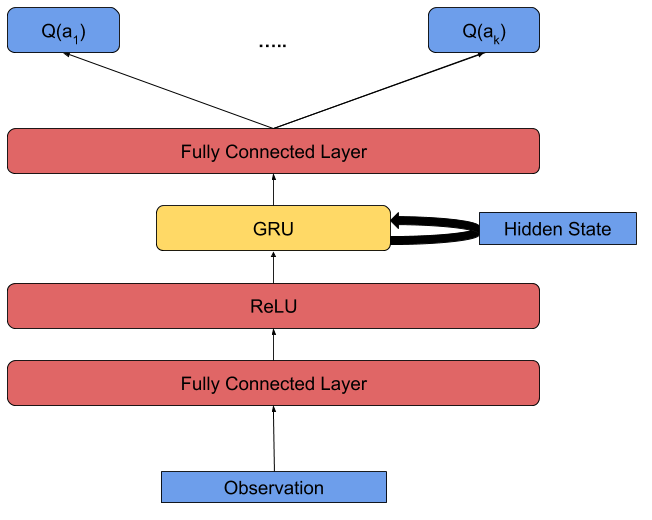
\includegraphics[scale=0.3]{images/agent_diagrams/rnn_agent_diagram.png}
    \caption{The standard \textit{rnn} architecture.}
    \label{fig:rnn_agent_diagram}
\end{figure}


A modification of this architecture is to pass each action as an input so that for each agent, batch element and action, a single $Q$ value is outputted, representing the $Q$ value of that particular action with the corresponding observation. This new architecture is illustrated in figure \ref{fig:rnn_input_action_agent_diagram}.


Passing actions as inputs in this way changes the shape of the network, with more neurons at the input side (to deal with the action as an input), and less neurons at the output side (we no longer output a $Q$ value for each action). This may have implications to the speed of training and overall peformance, and is therefore important to experiment with.

\begin{figure}
    \centering
    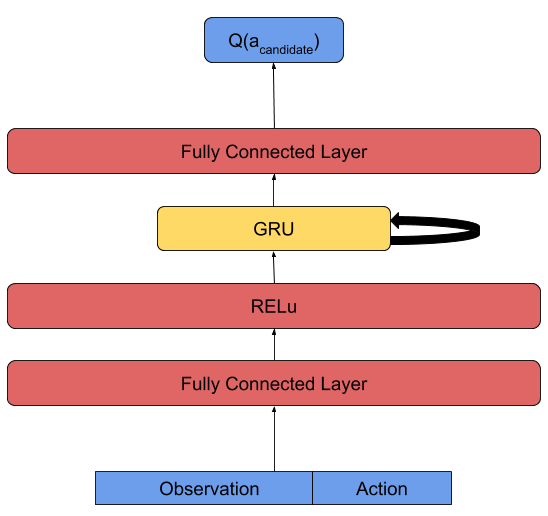
\includegraphics[scale=0.3]{images/agent_diagrams/rnn_input_action_agent_diagram.png}
    \caption{The \textit{rnn\_input\_action} architecture.}
    \label{fig:rnn_input_action_agent_diagram}
\end{figure}

\subsection{Grid Representation of Observations and Actions}

A relatively simple way to abstract an observation of a particular agent is to generate a grid (with the agent at the centre) with various channels containing relevant features, with each cell representing a location in this agent's field of view. The features may include whether a particular cell contains an ally or an enemy unit (or neither), the health of a unit and the type of a unit (Marine, Zealot etc.). 

We are also able to represent actions in a similar way. There are two main types of action we wish to consider: movement and attack. Therefore, two channels in the action grid are required to differentiate between the two. We can place a value of $1$ in the cell north, south, east or west of the agent we are considering (in the movement channel) to represent a movement in the respective direction. All other values will be zero, as we are only considering one action at a time. For attack, we place a value in the cell of the unit we are wanting to attack (in the attack channel), again with zeroes in all other cells.

In both of these cases, the grids are three dimensional tensors (in the PyTorch framework).

The reason for these style of observations is to allow for the use of convolutional neural networks to better find patterns in the graphical representation of the environment, as we will explore in the following section.

\subsubsection{Observation and Action Decoders}

Some key pieces of engineering to allow for the use of grid-based actions and observations are the action encoder and observation decoder. 

The action encoder turns Starcraft II actions (one-hot encoding) into grid actions (with 2 channels for movement and attack). In the action grid, the central cell represents the agent with respect to its field of view. If the action is a movement action, then a 1 is filled in the adjacent north south, east or west cell (depending on which direction the action is) in the movement channel. All other cells are left as 0. If the action is an attack action, then a 1 is filled in the cell in which the unit to attack is occupying, in the attack channel. Again, all other cells remain as 0. 

The observation decoder turns Starcraft II (one dimensional) observations into grid observations. Again, the agent is at the centre of the grid, and any observation concerning another unit is put into a channel of the cell at that unit's location.

The observation decoder and action encoder are both applied in the ``build\_inputs'' function, which is used to prepare the inputs before they are sent to the agent network. This allows the inputs to take the various forms as we will see in the candidate architectures. 

\subsubsection{Convolutional Neural Network Agents}

A possible way to enhance the performance of the simple RNN-based agent networks is to include convolutional layers in the network. This allows the agent network to make make stronger deductions about the relations between entities in each observation, and recognize patterns that would otherwise not be recognized, especially if observations and actions are represented as images (grid-based). 

The convolutional layers will form a convolutional encoder, that was originally shown to be successful in \cite{ddpg}, which explored the use of deep deterministic policy gradients (DDPG). The encoder is simply three convolutional layers, which have 32 filters each and no pooling. After each convolutional layer, an exponential linear unit is used as the activation function.

In contrast to ReLUs, ELUs have negative values which allows them to push mean unit activations closer to zero like batch normalization but with lower computational complexity. Mean shifts toward zero speed up learning by bringing the normal gradient closer to the unit natural gradient because of a reduced bias shift effect \cite{elu}.


We first consider a simple agent network using this convolutional encoder (as well as a GRU-cell, to allow for the same power as the previous RNNs). We first feed the grid-based observation into the convolutional encoder, before flattening the output into a 1-dimensional tensor. We do this to be able to concatenate the 1-dimensional observation information (agent identifier, last action performed etc.). The next layer is a fully connected linear layer, before a rectified linear unit as the nonlinearity. What follows is a GRU-cell and another fully-connected layer, which outputs a Q-value for each possible action. Intuitively, the convolutional encoder captures various information about the relation between entities in the observation, while the multiple fully-connected layers extract this information into the Q-values. The GRU-cell allows for the network to use information about the past time-series data, to give an even more informed result. We shall refer to this agent network as \textit{conv}. The architecture of this agent network is shown in figure \ref{fig:conv_agent_diagram}

\begin{figure}
    \centering
    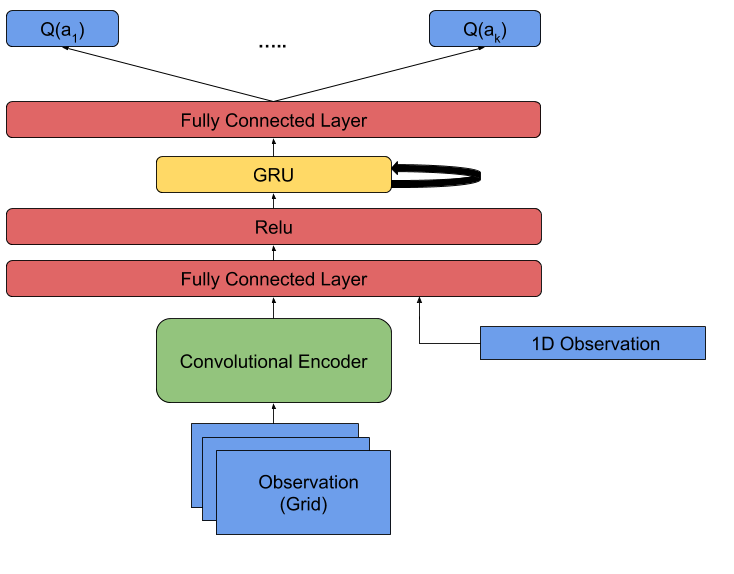
\includegraphics[scale=0.3]{images/agent_diagrams/rnn_conv_ddpg_agent_diagram.png}
    \caption{The \textit{conv} architecture.}
    \label{fig:conv_agent_diagram}
\end{figure}

As in \textit{rnn\_input\_action}, we can also experiment with the idea of using a candidate action as an input in order to output a single $Q$-value (for that observation and action pair), rather than simply have a $Q$-value for each possible action. This yields a new agent network, which inputs grid observations into the convolutional encoder as normal, but concatenates a candidate action onto the 1-dimensional encoded observation. The layers are the same as in conv, except that the last fully-connected linear layer has a single output, for the $Q$-value corresponding to the particular observation and action pair. We shall refer to this agent network architecture as \textit{conv\_input\_flat}. The architecture is shown in figure \ref{fig:conv_input_flat_diagram}.

\begin{figure}
    \centering
    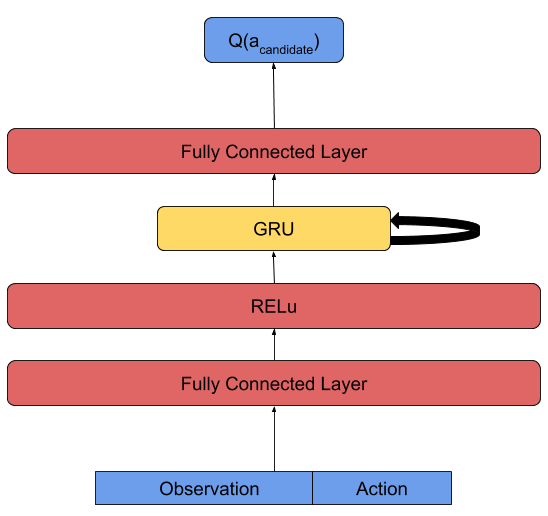
\includegraphics[scale=0.3]{images/agent_diagrams/rnn_input_action_agent_diagram.png}
    \caption{The \textit{conv\_input\_flat} architecture.}
    \label{fig:conv_input_flat_diagram}
\end{figure}


The previous two agent networks’ convolutional encoders do not encode any information about the possible actions, only the observations. Therefore, a possible change that can be made is to somehow include the actions (in their grid-based representations) as input into the encoder. This requires us to input actions into the network first, and receive a single Q-value for that particular observation and action pair, rather than receive a Q-value for each possible action, which is seen in \textit{rnn\_input\_action}. As described before, actions are represented in a similar way to observations, but with just 2 channels (movement and attack), with a single 1 in a cell to represent movement (or attack) to a particular location in the agents field of view. The architecture of this agent network is similar to that of conv, but the action grid representation is concatenated to the observation grid representation, and then is fed forward through the network as normal. We also only have a single output from the last fully connected linear layer, representing the Q-value of that particular observation and action pair. This agent network architecture is referred to as \textit{conv\_input\_grid}..

The architecture can be seen in figure \ref{fig:conv_input_grid_agent_diagram}.

\begin{figure}
    \centering
    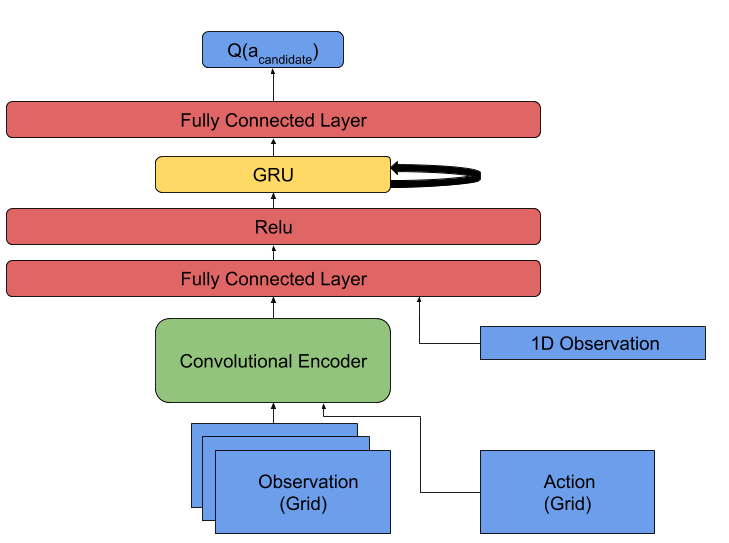
\includegraphics[scale=0.3]{images/agent_diagrams/rnn_conv_ddpg_input_grid_agent_diagram.png}
    \caption{The \textit{conv\_input\_grid} architecture.}
    \label{fig:conv_input_grid_agent_diagram}
\end{figure}





\subsection{Grid Size}

We are able to change the ``resolution'' of the observation (and action grid) by changing the width and height of the grid. The grid always covers only the field of view of the agent, but the number of cells in the grid (i.e. the ``resolution'') can be changed.  A larger number of cells in the grid gives a greater amount of detail, but also a greater amount of computation and more sparse images will be generated (which the network may have trouble extracting useful relationships from). Therefore, a balance has to be made. This will form a large part of the experiments for these agent networks.





\subsection{Problems Encountered}
In the implementation of these agent networks, there were multiple challenges to overcome.

\subsubsection{Multiple Occupancy}
A problem was encountered concerning multiple agents occupying a small area, so that the observation (and action) grid representation would try to represent multiple agents (or actions) in a single cell, which is not possible by the construction of such a representation. This is solved by first running a check for such a scenario, and, if the problem exists, repeatedly trying to reallocate the offending agents to a neighbouring cell until the problem is no longer there. Without this, multiple units in near proximity would be counted as a single unit, which would present a significant problem as the observation is far from complete. 

\subsubsection{Memory Usage}
Due to the differing complexities of the agent networks, there is a wide range of memory usage for them. In particular, it was found that the agent networks that use grid observations require a larger amount of GPU memory than those that don't, because the fully connected layers must be far larger in order to deal with the output of convolutional layers. This effect greater if the actions are also represented in grid form, as the number of channels in the tensor is further increased. 

Furthermore, the larger the grid size, the greater the GPU memory used.

On certain grid sizes, the high memory usage is so high (greater than 12Gb) that it causes the framework to terminate. Therefore, this problem must be resolved.

There are a number of ways to deal with this high memory usage. We could use a downsampling layer to reduce the output of the convolutional layers before the linear layers, to reduce the number of parameters. This was tried, but since the observations (and actions) are larger when in grid form, this approach was not very effective as it did not address the issue of the size of the observations. 

Therefore, another approach, which was far more effective in practice, was to reduce the batch size. There are two batch sizes that can be changed, the training batch size, and the running batch size. The training batch size controls how large the batches are that are sampled from the replay buffer. The running batch size controls how large the batches are that are inserted into the replay buffer. Therefore, reducing either of these will reduce the amount of memory required when sampling the replay buffer.

The batch size can have an impact on training performance: a larger batch size generally decreases the variance of the estimates of $Q$-values, allowing for more consistent gradient descent traversals. However, a lower batch size can introduce more noise in the sampling, and allows for escaping local minima, as well as avoiding overfitting.

With these considerations, in situations where memory usage is high, it is generally advisable for the batch size to be as large as possible before memory usage becomes too high.








\subsection{Making Architectures Independent of Number of Units}
A significant problem with the current architecture of all agent networks is the dependence on the number of units in the map. Currently, each unit in the field of view of an agent presents another possible action, which (if this action is represented as a tensor) fixes this architecture size. This is because the input (or output) of the network has to fit this action exactly, so the number of actions changes this. This independence is removed by representing actions as a grid, as seen in \textit{conv\_input\_grid}.

Furthermore, a common input to all network architectures is the agent's ID, whose size is dependent on the number of agents in the map. Again, this causes the architecture to be dependent on the number of agents. A possible way to resolve this issue is to simply drop this input. The network is still able to semi-identify the agent by its agent-type (Marine, Zealot etc.) (which is still input into the network). Of course, not inputting central information like the agent's identifier is likely to cause a drop in performance, it is important to evaluate the viability of architectures independent to the number of units on the map.

A huge advantage to network architectures which are independent of the number of units in the map is the idea of transfer learning. For example, training on the 3M map is fairly quick (around 6-12 hours on an RTX 2080 ti), but training on 30M is much longer (time for training on 30M). It may be possible to reach a reasonable level of ability by first training on smaller (but similar) maps, and using this model on the larger map.


Therefore, we can produce a final agent network, which will be used solely to experiment with this idea, by removing the agent ID input from \textit{conv\_input\_grid}. This agent network architecture is referred to as \textit{conv\_input\_grid\_no\_id}.


The comparison of this agent network with others will form a significant part of the experiments section in order to evaluate the importance of particular information during training, as well as seeing if architecture independent to the number of units is a viable mechanism that can be used for transfer learning.

